\documentclass[12pt, a4paper]{article}

% ==================== Pacotes ====================
\usepackage[utf8]{inputenc}
\usepackage[T1]{fontenc}
\usepackage[brazilian]{babel}
\usepackage{amsmath, amssymb, amsfonts}
\usepackage{graphicx}
\usepackage{booktabs}
\usepackage{float}
\usepackage[margin=2.5cm]{geometry}
\usepackage{caption}
\usepackage{subcaption}
\usepackage{hyperref}
\usepackage{indentfirst}

% ==================== Informações do Documento ====================
\title{Projeto 1 --- MS211 \\[0.3cm]
\large Cálculo Numérico}

\author{
    João Francisco Silva Freitas --- RA: 281254 \\
    Matheus Yanetti Carvalhal Franca Menezes --- RA: XXXXXX\\
}

\date{Outubro de 2026}

\begin{document}

\maketitle

% ==================== Introdução ====================
\section*{Introdução}

Neste projeto, desenvolvemos por completo as seguintes seções do roteiro:

\begin{itemize}
    \item \textbf{Seção 2:} Zeros de funções de uma variável real.
    \item \textbf{Seção X:} \textit{(a ser preenchido com a segunda seção escolhida)}.
\end{itemize}

Toda a implementação numérica foi realizada em Python, sem o uso de bibliotecas de solvers automáticos.
Utilizamos apenas \texttt{NumPy} para manipulação de vetores, \texttt{Pandas} para geração de tabelas e \texttt{Matplotlib} para visualização gráfica, conforme permitido pelo enunciado.


% ======================================================================
%                       SEÇÃO 2 — ZEROS DE FUNÇÕES
% ======================================================================
\newpage
\section{Seção 2 --- Zeros de Funções de Uma Variável}

Nesta seção, implementamos os métodos da Bissecção, de Newton e da Secante para a determinação de zeros de funções reais de uma variável. Investigamos dois casos: o primeiro compara a eficiência e a taxa de convergência dos três métodos para um polinômio cúbico; o segundo explora a natureza \emph{local} da convergência do método de Newton aplicado à função arco-tangente.


% ======================== CASO 1 ========================
\subsection{Caso 1 --- Comparação de Convergência}

Consideramos a função polinomial:
\begin{equation}
    f(x) = x^3 - 3x + 1
\end{equation}


\subsubsection*{(a) Existência, unicidade e valor analítico da raiz em $[1, 2]$}

\paragraph{Existência (Teorema do Valor Intermediário).}
A função $f$ é contínua em $[1, 2]$ por ser polinomial. Calculando os valores nos extremos do intervalo:
\[
    f(1) = 1 - 3 + 1 = -1 < 0, \qquad f(2) = 8 - 6 + 1 = 3 > 0.
\]
Como $f(1) < 0$ e $f(2) > 0$, pelo Teorema do Valor Intermediário, existe pelo menos um zero de $f$ no intervalo $(1, 2)$.

\paragraph{Unicidade.}
A derivada de $f$ é dada por $f'(x) = 3x^2 - 3 = 3(x-1)(x+1)$.
Para todo $x \in (1, 2]$, temos $x - 1 > 0$ e $x + 1 > 0$, logo $f'(x) > 0$.
Como $f$ é contínua em $[1, 2]$ e $f'(x) > 0$ para $x \in (1, 2]$, a função é estritamente crescente nesse intervalo e, portanto, injetora. Logo, existe \textbf{no máximo} uma raiz em $[1, 2]$. Combinando com a existência provada pelo TVI, concluímos que existe \textbf{exatamente uma} raiz $\alpha \in (1, 2)$.

\paragraph{Cálculo analítico via mudança de variável.}
Utilizando a substituição $x = 2\cos\theta$ e a identidade $\cos(3\theta) = 4\cos^3\theta - 3\cos\theta$:
\begin{align}
    f(x) &= 8\cos^3\theta - 6\cos\theta + 1 = 2(4\cos^3\theta - 3\cos\theta) + 1 \notag \\
         &= 2\cos(3\theta) + 1.
\end{align}
Assim:
\[
    f(x) = 0 \iff 2\cos(3\theta) + 1 = 0 \iff \cos(3\theta) = -\frac{1}{2}.
\]
Como $\alpha \in [1, 2]$, temos $\alpha/2 \in [1/2, 1]$, logo existe um único $\theta \in [0, \pi/3]$ tal que $\alpha = 2\cos\theta$. Neste intervalo, a solução é:
\[
    3\theta = \frac{2\pi}{3} \implies \theta = \frac{2\pi}{9} \implies \boxed{\alpha = 2\cos\!\left(\frac{2\pi}{9}\right) \approx 1{,}5320888862}.
\]


\subsubsection*{(b) Aplicação dos métodos numéricos}

Aplicamos os três métodos com tolerância $\text{tol} = 10^{-10}$ e os seguintes parâmetros iniciais:
\begin{itemize}
    \item \textbf{Bissecção:} $a = 1$, $b = 2$. Critério de parada: $\frac{|b - a|}{2} < \text{tol}$.
    \item \textbf{Newton:} $x_0 = 2$. Critério de parada: $|x_{k+1} - x_k| < \text{tol}$.
    \item \textbf{Secante:} $x_0 = 1$, $x_1 = 2$. Critério de parada: $|x_{k+1} - x_k| < \text{tol}$.
\end{itemize}


\subsubsection*{(c) Tabelas dos iterados}

\begin{table}[H]
    \centering
    \caption{Iterados do Método de Newton ($x_0 = 2$).}
    \label{tab:newton}
    \begin{tabular}{rrrr}
\toprule
k & x_k & |f(x_k)| & |x_k - alpha| \\
\midrule
0 & 2.0000000000 & 3.0000e+00 & 4.6791e-01 \\
1 & 1.6666666667 & 6.2963e-01 & 1.3458e-01 \\
2 & 1.5486111111 & 6.8040e-02 & 1.6522e-02 \\
3 & 1.5323901619 & 1.2181e-03 & 3.0128e-04 \\
4 & 1.5320889894 & 4.1696e-07 & 1.0316e-07 \\
5 & 1.5320888862 & 4.8406e-14 & 1.1990e-14 \\
6 & 1.5320888862 & 4.4409e-16 & 0.0000e+00 \\
\bottomrule
\end{tabular}

\end{table}

\begin{table}[H]
    \centering
    \caption{Iterados do Método da Secante ($x_0 = 1$, $x_1 = 2$).}
    \label{tab:secante}
    \begin{tabular}{rrrr}
\toprule
k & x_k & |f(x_k)| & |x_k - alpha| \\
\midrule
0 & 1.0000000000 & 1.0000e+00 & 5.3209e-01 \\
1 & 2.0000000000 & 3.0000e+00 & 4.6791e-01 \\
2 & 1.2500000000 & 7.9688e-01 & 2.8209e-01 \\
3 & 1.4074074074 & 4.3444e-01 & 1.2468e-01 \\
4 & 1.5960829579 & 2.7774e-01 & 6.3994e-02 \\
5 & 1.5225014665 & 3.8330e-02 & 9.5874e-03 \\
6 & 1.5314246225 & 2.6829e-03 & 6.6426e-04 \\
7 & 1.5320961972 & 2.9550e-05 & 7.3110e-06 \\
8 & 1.5320888807 & 2.2335e-08 & 5.5258e-09 \\
9 & 1.5320888862 & 1.8474e-13 & 4.5741e-14 \\
10 & 1.5320888862 & 4.4409e-16 & 0.0000e+00 \\
\bottomrule
\end{tabular}

\end{table}

\begin{table}[H]
    \centering
    \caption{Resumo comparativo dos três métodos.}
    \label{tab:resumo}
    \begin{tabular}{lrrlll}
\toprule
Método & Iterações & Avaliações f & Avaliações f' & Erro Final & Resíduo Final \\
\midrule
Bissecção & 34 & 35 & — & 4.8216e-11 & 1.9488e-10 \\
Secante & 9 & 10 & — & 0.0000e+00 & 4.4409e-16 \\
Newton & 6 & 6 & 6 & 0.0000e+00 & 4.4409e-16 \\
\bottomrule
\end{tabular}

\end{table}

\paragraph{Observações.}
A tabela completa da Bissecção possui 34 iterados e foi omitida por brevidade; o resultado final e as contagens constam na Tabela~\ref{tab:resumo}. Nota-se que:
\begin{itemize}
    \item O método de \textbf{Newton} convergiu em apenas \textbf{6 iterações} (6 avaliações de $f$ e 6 de $f'$), atingindo erro de máquina.
    \item O método da \textbf{Secante} convergiu em \textbf{9 iterações} (10 avaliações de $f$), sem necessidade de calcular derivadas.
    \item A \textbf{Bissecção} convergiu em \textbf{34 iterações} (35 avaliações de $f$), sendo o mais lento dos três, como esperado pela teoria.
\end{itemize}


\subsubsection*{(d) Gráfico de dígitos corretos e ordem assintótica}

Definimos $d_k = -\log_{10}|x_k - \alpha|$ para os iterados tais que $x_k \neq \alpha$. Essa grandeza representa, intuitivamente, o número de dígitos decimais corretos da aproximação $x_k$.

\begin{figure}[H]
    \centering
    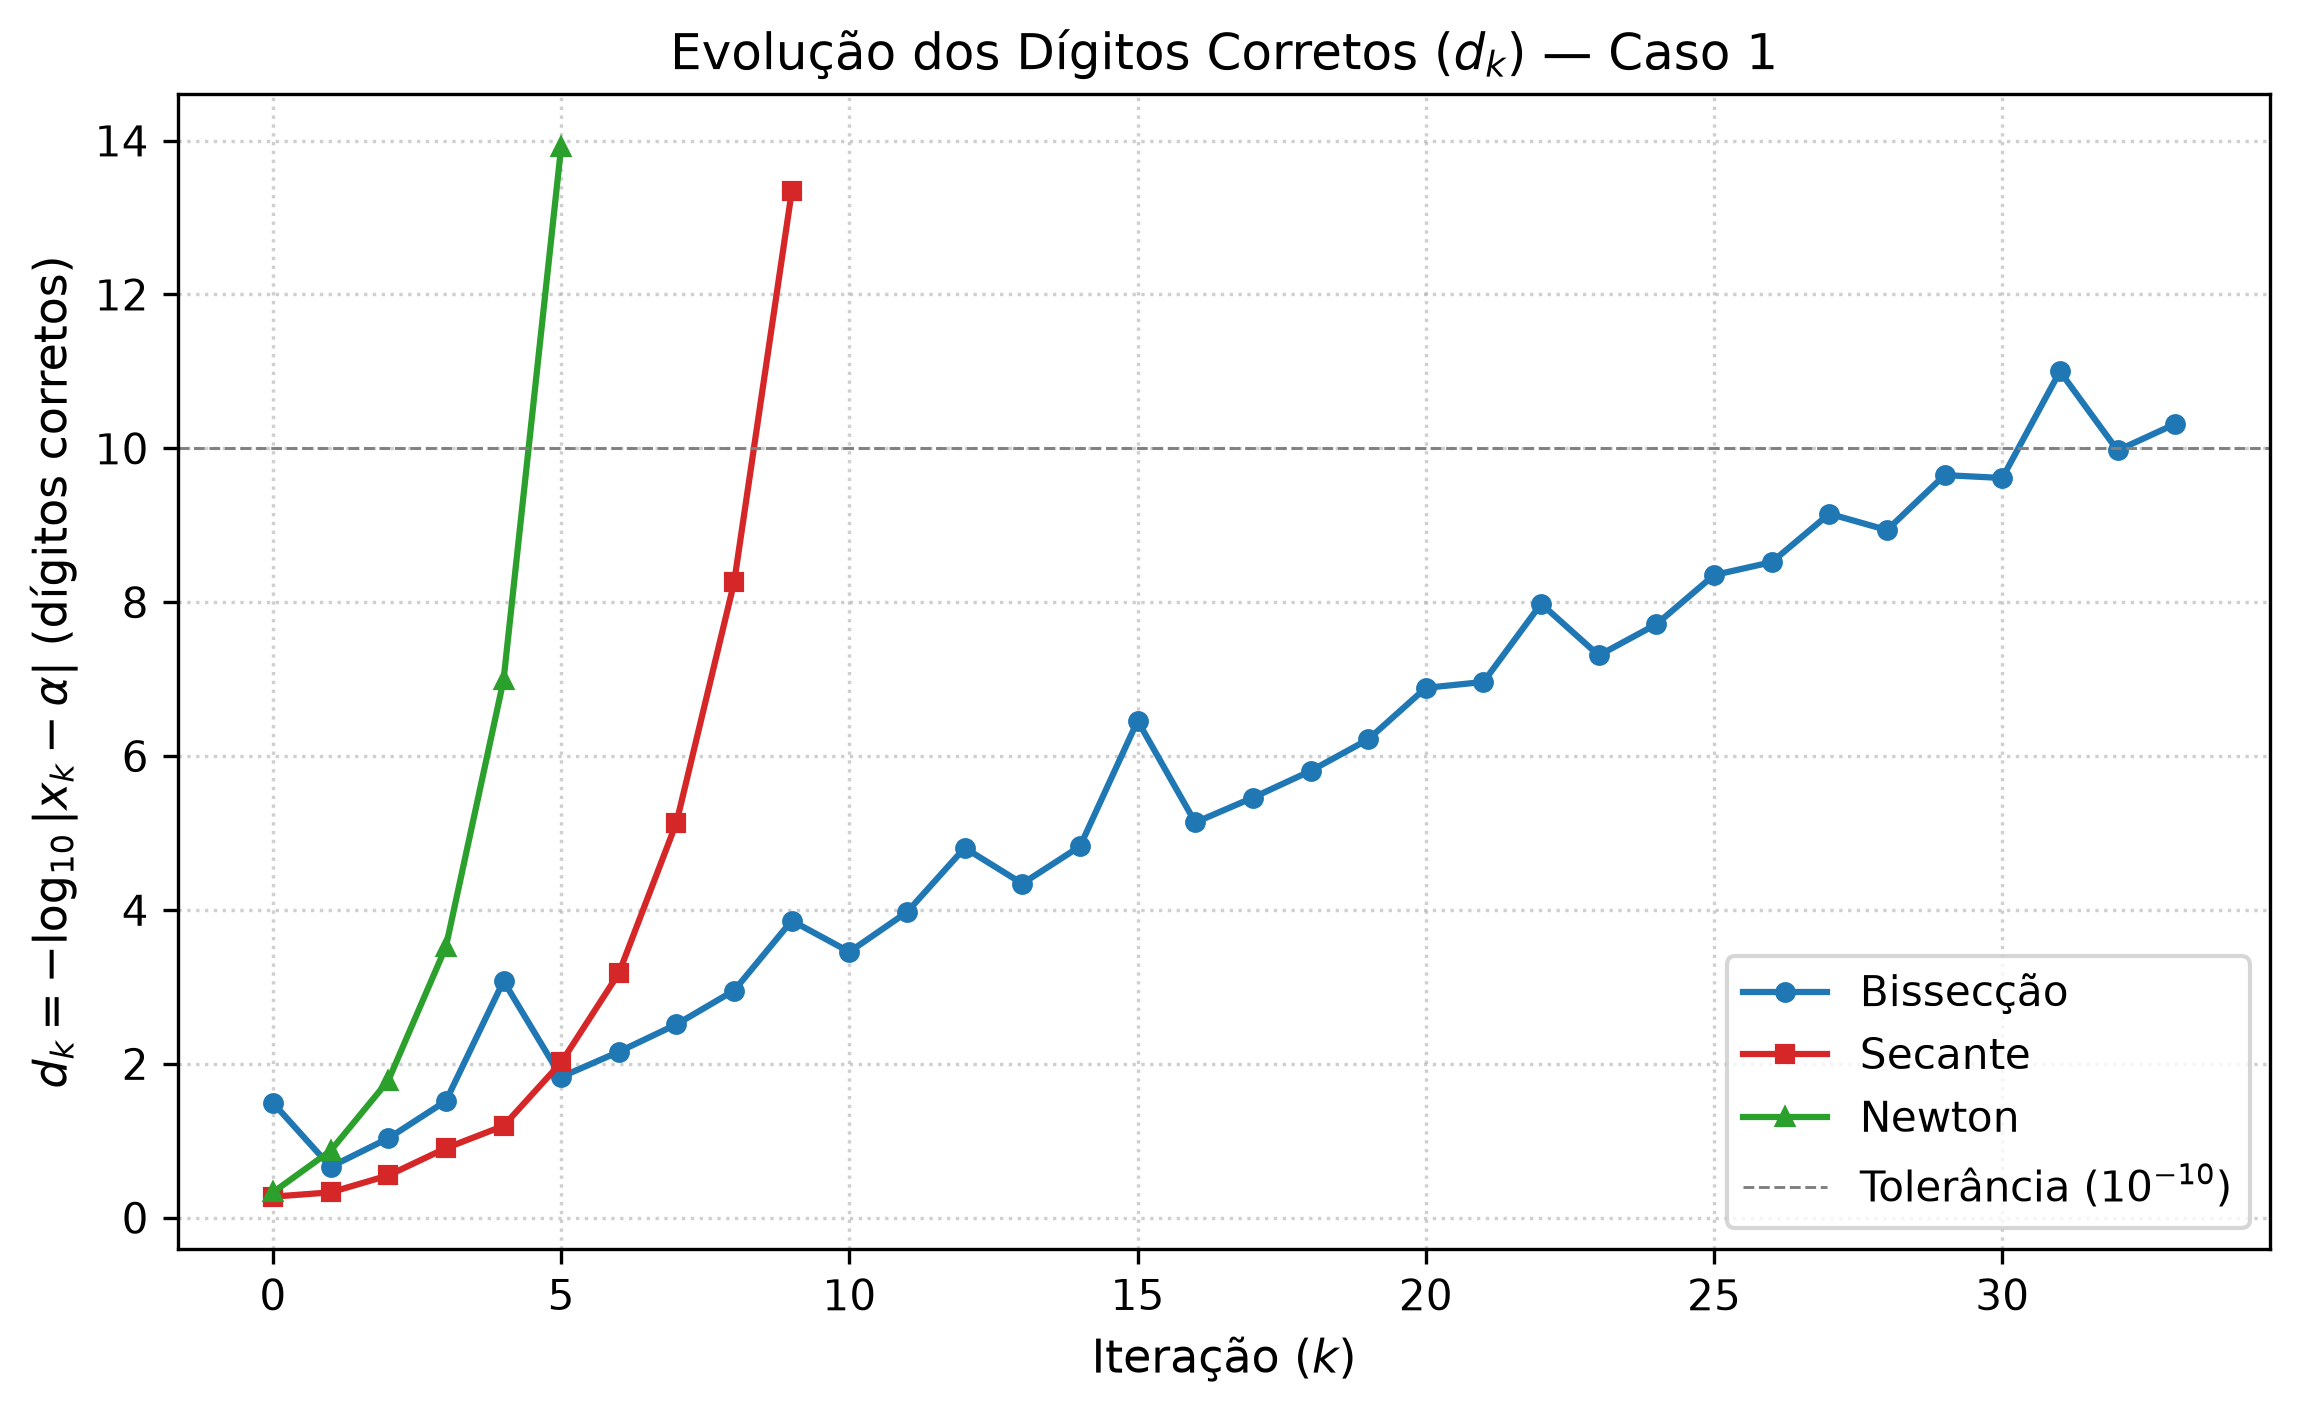
\includegraphics[width=0.85\textwidth]{../tema2/grafico_dk_caso1.png}
    \caption{Evolução dos dígitos corretos $d_k$ em função da iteração $k$ para os três métodos. A linha tracejada indica a tolerância $10^{-10}$ ($d_k = 10$).}
    \label{fig:dk_caso1}
\end{figure}

\paragraph{Análise do gráfico.}
A Figura~\ref{fig:dk_caso1} evidencia claramente as diferentes velocidades de convergência:
\begin{itemize}
    \item \textbf{Bissecção:} $d_k$ cresce linearmente com inclinação $\approx \log_{10}(2) \approx 0{,}301$, ou seja, ganha-se cerca de 1 casa decimal a cada 3,3 iterações. Isso confirma a taxa de convergência \emph{linear} esperada.
    \item \textbf{Secante:} a curva de $d_k$ apresenta curvatura para cima, acelerando a cada iteração, compatível com a convergência \emph{superlinear} de ordem $\varphi = (1 + \sqrt{5})/2 \approx 1{,}618$.
    \item \textbf{Newton:} a curva dispara quase verticalmente, dobrando o número de casas decimais corretas a cada iteração, o que reflete a convergência \emph{quadrática} teórica.
\end{itemize}

\paragraph{Estimativa da ordem assintótica.}
Para Newton e Secante, estimamos a ordem de convergência pela fórmula:
\[
    p_k = \frac{\ln\!\left(\left|e_{k+1}\right|/\left|e_k\right|\right)}
              {\ln\!\left(\left|e_k\right|/\left|e_{k-1}\right|\right)},
    \quad \text{onde } e_k = x_k - \alpha.
\]
Utilizamos apenas índices $k$ para os quais os erros não estejam dominados pelo arredondamento de ponto flutuante ($|e_k| > 10^{-14}$).

\begin{table}[H]
    \centering
    \caption{Estimativa da ordem assintótica $p_k$ para Newton e Secante.}
    \label{tab:pk}
    \begin{tabular}{c c c}
        \toprule
        $k$ & $p_k$ (Newton) & $p_k$ (Secante) \\
        \midrule
        1 & 1,6832 & 3,9372 \\
        2 & 1,9092 & 1,6134 \\
        3 & 1,9927 & 0,8169 \\
        4 & 2,0011 & 2,8462 \\
        5 & ---    & 1,4062 \\
        6 & ---    & 1,6892 \\
        7 & ---    & 1,5940 \\
        8 & ---    & 1,6281 \\
        \bottomrule
    \end{tabular}
\end{table}

\paragraph{Conclusão.}
Para o método de \textbf{Newton}, os valores de $p_k$ convergem rapidamente para $2{,}0$, confirmando a convergência \emph{quadrática} prevista pela teoria (raiz simples com $f'(\alpha) \neq 0$).

Para o método da \textbf{Secante}, os valores finais de $p_k$ oscilam em torno de $1{,}62$, concordando excelentemente com a previsão teórica de $p = \varphi \approx 1{,}618$ (razão áurea). Os valores iniciais oscilam porque a Secante requer um número maior de iterações para que a estimativa assintótica se estabilize (o comportamento pré-assintótico depende da qualidade das aproximações iniciais $x_0$ e $x_1$).


% ======================== CASO 2 ========================
\subsection{Caso 2 --- Localidade do Método de Newton}

Consideramos agora a função:
\begin{equation}
    g(x) = \arctan(x),
\end{equation}
cuja única raiz é $\alpha = 0$. A derivada é $g'(x) = \dfrac{1}{1 + x^2}$.


\subsubsection*{(a) Fórmula de recorrência e comportamento para diferentes $x_0$}

A iteração de Newton para $g$ assume a forma:
\begin{equation}
    x_{k+1} = x_k - \frac{g(x_k)}{g'(x_k)} = x_k - (1 + x_k^2)\arctan(x_k).
    \label{eq:newton_arctg}
\end{equation}

Executamos 10 iterações para seis aproximações iniciais: $x_0 \in \{0{,}5;\; 1{,}0;\; 1{,}3;\; 1{,}4;\; 1{,}5;\; 2{,}0\}$. Os resultados são apresentados na Tabela~\ref{tab:caso2_iterados}.

\begin{table}[H]
    \centering
    \caption{Iterados do método de Newton para $g(x) = \arctan(x)$ com diferentes $x_0$.}
    \label{tab:caso2_iterados}
    \resizebox{\textwidth}{!}{\begin{tabular}{rrrrrrr}
\toprule
k & x0=0.5 & x0=1 & x0=1.3 & x0=1.4 & x0=1.5 & x0=2 \\
\midrule
0 & 5.0000e-01 & 1.0000e+00 & 1.3000e+00 & 1.4000e+00 & 1.5000e+00 & 2.0000e+00 \\
1 & -7.9560e-02 & -5.7080e-01 & -1.1616e+00 & -1.4136e+00 & -1.6941e+00 & -3.5357e+00 \\
2 & 3.3530e-04 & 1.1686e-01 & 8.5890e-01 & 1.4501e+00 & 2.3211e+00 & 1.3951e+01 \\
3 & -2.5131e-11 & -1.0610e-03 & -3.7424e-01 & -1.5506e+00 & -5.1141e+00 & -2.7934e+02 \\
4 & 0.0000e+00 & 7.9631e-10 & 3.4019e-02 & 1.8471e+00 & 3.2296e+01 & 1.2202e+05 \\
5 & 0.0000e+00 & 0.0000e+00 & -2.6240e-05 & -2.8936e+00 & -1.5753e+03 & -2.3386e+10 \\
6 & 0.0000e+00 & 0.0000e+00 & 1.2045e-14 & 8.7103e+00 & 3.8950e+06 & 8.5908e+20 \\
7 & 0.0000e+00 & 0.0000e+00 & 0.0000e+00 & -1.0325e+02 & -2.3830e+13 & -1.1593e+42 \\
8 & 0.0000e+00 & 0.0000e+00 & 0.0000e+00 & 1.6541e+04 & 8.9203e+26 & 2.1110e+84 \\
9 & 0.0000e+00 & 0.0000e+00 & 0.0000e+00 & -4.2972e+08 & -1.2499e+54 & -6.9999e+168 \\
10 & 0.0000e+00 & 0.0000e+00 & 0.0000e+00 & 2.9006e+17 & 2.4540e+108 & inf \\
\bottomrule
\end{tabular}
}
\end{table}

\paragraph{Análise qualitativa.}
A Tabela~\ref{tab:caso2_iterados} e a Figura~\ref{fig:caso2_semilog} revelam dois comportamentos nitidamente distintos:
\begin{itemize}
    \item Para $x_0 \in \{0{,}5;\; 1{,}0;\; 1{,}3\}$: os iterados convergem rapidamente para a raiz $\alpha = 0$, atingindo precisão de máquina em poucas iterações.
    \item Para $x_0 \in \{1{,}4;\; 1{,}5;\; 2{,}0\}$: os iterados divergem com amplitude crescente e \emph{sinal alternante}, com $|x_k|$ crescendo exponencialmente (ou mais rapidamente) a cada iteração.
\end{itemize}

Isso sugere a existência de um valor limiar $x^* \in (1{,}3;\; 1{,}4)$ que separa os dois regimes.

\begin{figure}[H]
    \centering
    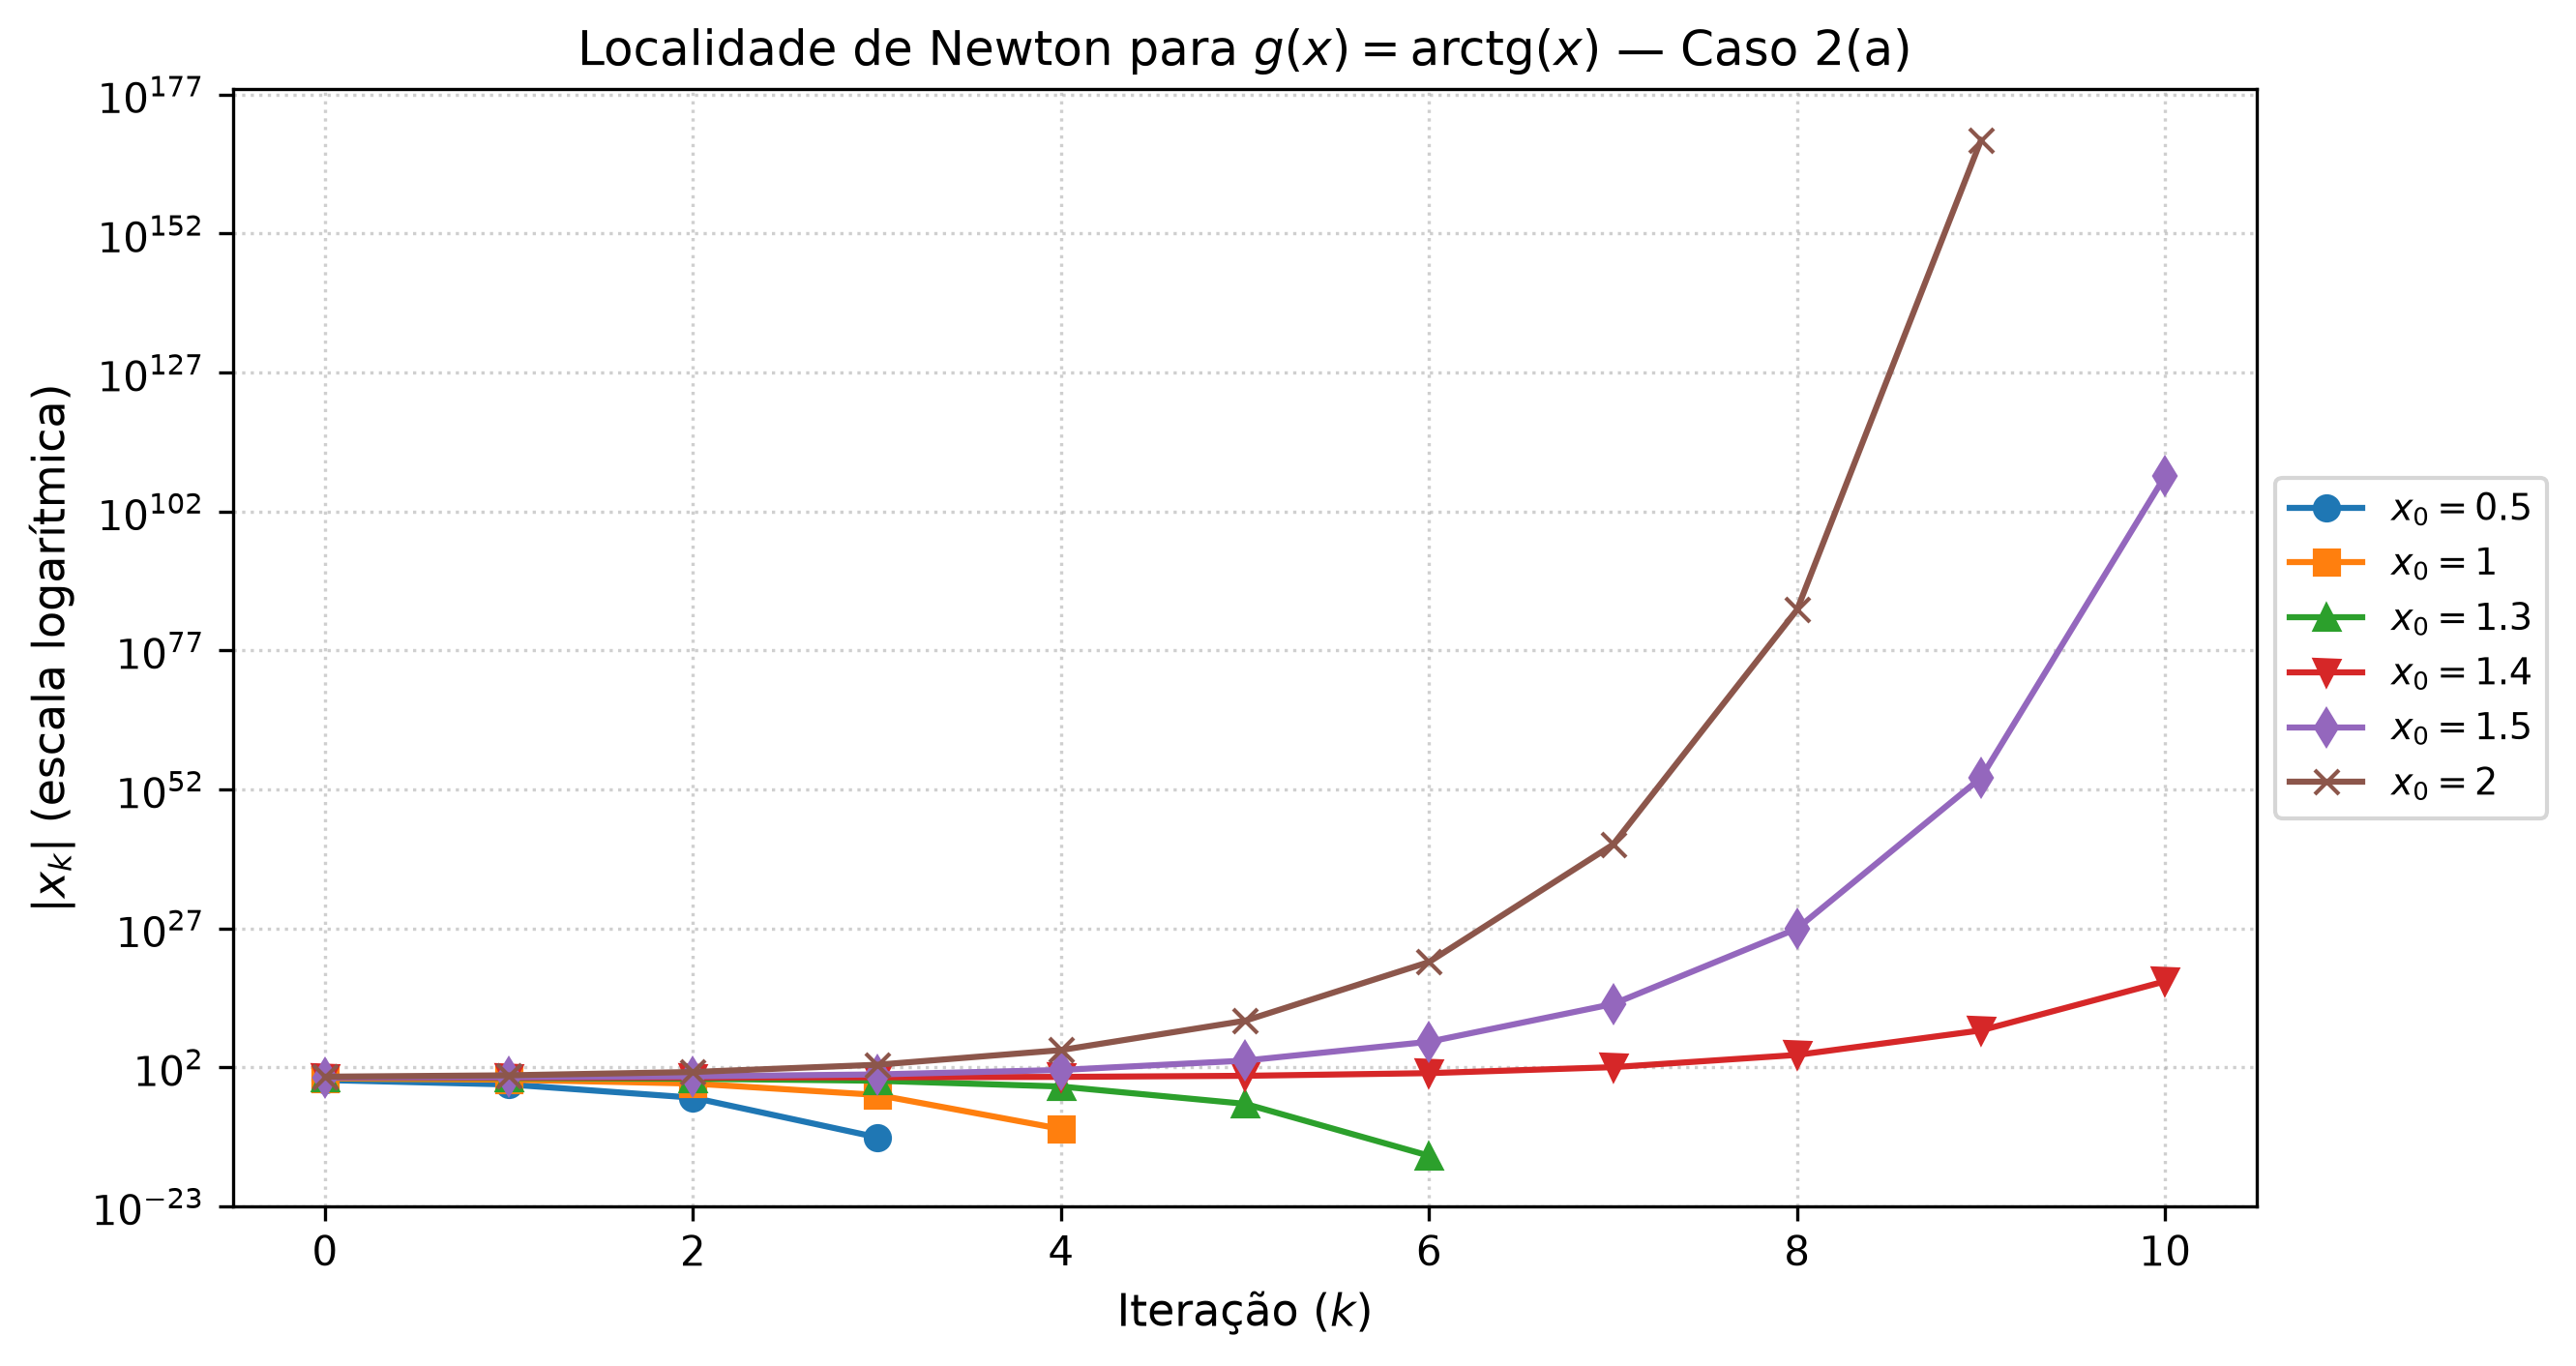
\includegraphics[width=0.85\textwidth]{../tema2/grafico_caso2_semilog.png}
    \caption{Módulo dos iterados $|x_k|$ em escala semilogarítmica para as seis aproximações iniciais. As curvas que descem correspondem a convergência; as que sobem, a divergência oscilatória.}
    \label{fig:caso2_semilog}
\end{figure}


\subsubsection*{(b) Determinação do ponto limiar $x^*$}

O limiar de estabilidade corresponde ao valor $x^* > 0$ para o qual a iteração de Newton produz exatamente o simétrico: $x_1 = -x_0$, formando um \emph{ciclo de período 2}. Impondo $-x^* = x^* - (1 + (x^*)^2)\arctan(x^*)$:
\begin{equation}
    h(x) \coloneqq 2x - (1 + x^2)\arctan(x) = 0.
    \label{eq:h_ciclo}
\end{equation}

Verificamos que $h(1) = 2 - 2\arctan(1) = 2 - \pi/2 \approx 0{,}429 > 0$ e $h(1{,}5) \approx -0{,}417 < 0$, garantindo pelo TVI a existência de uma raiz em $(1, 1{,}5)$.

Aplicando o método da \textbf{Bissecção} à equação~\eqref{eq:h_ciclo} no intervalo $[1, 1{,}5]$ com $\text{tol} = 10^{-10}$, obtivemos:
\[
    \boxed{x^* \approx 1{,}3917452003}
\]
em 33 iterações da bisseção, com resíduo $|h(x^*)| \approx 8{,}48 \times 10^{-11}$.

Isso confirma quantitativamente que a transição entre convergência e divergência observada na Tabela~\ref{tab:caso2_iterados} ocorre no intervalo $(1{,}3;\; 1{,}4)$.


\subsubsection*{(c) Análise dos três regimes}

Testamos o método de Newton com 25 iterações para valores representativos de cada regime:

\paragraph{Regime 1: $|x_0| < x^*$ (convergência para zero).}
Para $x_0 = 1{,}20$ e $x_0 = 1{,}35$, os iterados convergem rapidamente para a raiz $\alpha = 0$, atingindo o zero de máquina em 6 e 8 iterações, respectivamente.
Isso confirma que, para $|x_0| < x^*$, o método de Newton converge localmente, como garantido pelo teorema de convergência local.

\paragraph{Regime 2: $|x_0| = x^*$ (ciclo de período 2).}
Para $x_0 = x^*$ e $x_0 = -x^*$, os iterados iniciam alternando entre $+x^*$ e $-x^*$, formando o ciclo previsto pela equação~\eqref{eq:h_ciclo}. Entretanto, a partir de aproximadamente $k \approx 12$, os erros de arredondamento de ponto flutuante começam a ser amplificados a cada ciclo completo, e a trajetória se desestabiliza progressivamente: por volta de $k = 20$, os iterados já divergem de forma irrecuperável.

Este comportamento confirma que o ciclo de período 2 é um \textbf{ponto fixo instável} do mapa de dois passos $F(x) = N(N(x))$, onde $N$ é a iteração de Newton~\eqref{eq:newton_arctg}. A derivada do mapa de dois passos satisfaz $|F'(x^*)| > 1$, de modo que qualquer perturbação (incluindo os inevitáveis erros de arredondamento da aritmética de precisão finita) é amplificada exponencialmente, rompendo o ciclo.

\paragraph{Regime 3: $|x_0| > x^*$ (divergência oscilatória).}
Para $x_0 = 1{,}45$ e $x_0 = 1{,}80$, os iterados divergem imediatamente com amplitude crescente e sinal alternante, atingindo overflow ($|x_k| > 10^{308}$) em poucas iterações. Esse regime é completamente exterior à bacia de atração da raiz $\alpha = 0$.

\paragraph{Conclusão do Caso 2.}
Este experimento demonstra de forma concreta que o método de Newton é um método \emph{local}: a convergência para a raiz $\alpha = 0$ é garantida apenas quando $|x_0| < x^* \approx 1{,}3917$, ou seja, quando a aproximação inicial está suficientemente próxima da raiz. Para $|x_0| \geq x^*$, o método falha --- seja por entrar em um ciclo instável, seja por divergir oscilatoriamente.

A existência do ciclo de período 2 e sua instabilidade numérica reforçam a importância de se considerar o \emph{raio de convergência} do método e os efeitos da aritmética de ponto flutuante na análise de estabilidade de iterações numéricas.


% ======================================================================
%            SEÇÃO X — (segunda seção a ser desenvolvida)
% ======================================================================
\newpage
\section{Seção X --- \textit{(a ser preenchido)}}

\textit{Conteúdo da segunda seção escolhida será inserido aqui.}


\end{document}
